\documentclass{article}[11pt]
\usepackage[
  a4paper,
  margin = 15mm,
]{geometry}
\usepackage[disable]{todonotes}
%\usepackage[utf8]{inputenc}
%\usepackage[english, frenchb]{babel}
\usepackage{amssymb}
\usepackage{amsmath}
\usepackage{color}
\usepackage{pgfgantt}
\usepackage{hyperref}
\usepackage{fancyhdr}
\usepackage{xspace}
\usepackage{colortbl}
\usepackage{enumitem}
\usepackage{bussproofs}
\usepackage{tabu}
\setlength{\marginparwidth}{1.2cm}

%\usepackage[style=numeric,sorting=ydnt,defernumbers=true]{biblatex}
%\addbibresource{bib.bib}

\newcommand\BLL{BLL\xspace}
\newcommand\DlPCF{D$_\ell$PCF\xspace}
\newcommand\DFuzz{DFuzz\xspace}
\newcommand\rta{\rightarrow}
\newcommand\sS{\mathcal S}


\newganttlinktype{rd}{
\ganttsetstartanchor{on right}
\ganttsetendanchor{on top}
\draw[/pgfgantt/link]
(\xLeft, \yUpper) --
% second segment (right)
(\xRight, \yUpper) --
(\xRight, \yLower);
}
\newganttlinktype{ru}{
\ganttsetstartanchor{on right}
\ganttsetendanchor{on bottom}
\draw[/pgfgantt/link]
(\xLeft, \yUpper) --
% second segment (right)
(\xRight, \yUpper) --
(\xRight, \yLower);
}
\newganttlinktype{rus}{
\ganttsetstartanchor{on right}
\ganttsetendanchor{on bottom=0.3}
\draw[/pgfgantt/link]
(\xLeft, \yUpper) --
% second segment (right)
(\xRight, \yUpper) --
(\xRight, \yLower);
}
\newganttlinktype{rr}{
\ganttsetstartanchor{on right}
\ganttsetendanchor{on left}
\draw[/pgfgantt/link]
(\xLeft, \yUpper) --
% second segment (right)
(\xLeft, \yLower) --
(\xRight, \yLower);
}
\newganttlinktype{uu}{
\ganttsetstartanchor{on top=1}
\ganttsetendanchor{on bottom=0.753}
\draw[/pgfgantt/link]
(\xLeft, \yUpper) --
(\xRight, \yLower);
}
\newganttlinktype{uus}{
\ganttsetstartanchor{on top=1}
\ganttsetendanchor{on bottom=0.336}
\draw[/pgfgantt/link]
(\xLeft, \yUpper) --
(\xRight, \yLower);
}
\newganttlinktype{dd}{
\ganttsetstartanchor{on bottom=1}
\ganttsetendanchor{on top=0.753}
\draw[/pgfgantt/link]
(\xLeft, \yUpper) --
(\xRight, \yLower);
}

\pagestyle{fancyplain}
\lhead{}
\chead{{\color{gray}SATIR - GF}}
\rhead{}
\lfoot{{\color{gray}SATIR - Part B}}
\cfoot{}
\rfoot{{\color{gray}\thepage\ of \pageref{LastPage}}}


\title{SATIR\\ Statical Analysis via Type InfeRence}



\begin{document}

\begin{titlepage} 
  \vspace*{1.5cm}%\stretch{1.0}}
  \begin{center}
    \textsc{\huge\bf Start Page}\\[1.5cm]
    \textsc{\huge MARIE SKŁODOWSKA-CURIE ACTIONS}\\[1.5cm]
    \textsc{\bf\LARGE Individual Fellowships (IF)}\\
    \textsc{\bf\LARGE Call: H2020-MSCA-IF-2015}\\[1.5cm]
    \textsc{\LARGE PART B}\\[4cm] 
    \textsc{\Huge ``SATIR''}\\[0.5cm]
    \textsc{\LARGE ``Static Analysis via Type InfeRence''}\\[9cm]
    \textsc{\LARGE This proposal is to be evaluated as:}\\[0.5cm]
    \textsc{\LARGE [Global Fellowship (GF)]}
  \end{center} 
\end{titlepage}

\tableofcontents


\section*{List of Participants}

{\tabulinesep=1.2mm
  \begin{tabu}{| c | c | c | c | c | c | c | >{\columncolor[gray]{0}} c |}
    \hline
    \cellcolor[gray]{0.8} {\bf Participants} 
    & \cellcolor[gray]{0.8} \parbox[c]{4em}{\bf Legal Entity Short Name}
    & \cellcolor[gray]{0.8} \parbox[c]{1em}{\rotatebox[origin=c]{90}{\bf Academic}}\parbox[t]{1em}{\rotatebox[origin=c]{90}{(tick)}} 
    & \cellcolor[gray]{0.8} \parbox[c]{1em}{\rotatebox[origin=c]{90}{\bf non-Academic}}\parbox[t]{1em}{\rotatebox[origin=c]{90}{(tick)}}
    &  \cellcolor[gray]{0.8} {\bf Country} 
    & \cellcolor[gray]{0.8} \parbox[c]{6em}{\bf Dept./ Division/ Laboratory}
    &  \cellcolor[gray]{0.8} {\bf Supervisor}
    & \cellcolor[gray]{0.8} \parbox[c]{4em}{\bf Role of partner organisation} \\
    \hline
    \underline{Outgoing host} &&&&&&&\\
    \hline
    \parbox[c]{6em}{University of Pennsylvania} 
    & UPenn 
    & \checkmark
    && USA 
    & \parbox[c]{7em}{Department of Computer and Information Science} 
    & Steve Zdancewic &  \\
    & 
\includegraphics[angle=0,origin=c,scale=0.35]{UPenn.jpeg}
    &&&&&  
\includegraphics[angle=0,origin=c,scale=0.12]{stevez-fa15.jpg} & \\
    \hline
    \underline{Return host} &&&&&&&\\
    \hline
    \parbox[c]{6em}{University of Birmingham} 
    & Bham
    & \checkmark
    && UK 
    & \parbox[c]{7em}{School of Computer Science} 
    & Dan R. Ghica &  \\
    & 
\includegraphics[angle=0,origin=c,scale=0.3]{Bghm.jpeg}
    &&&&&  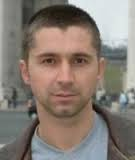
\includegraphics[angle=0,origin=c,scale=0.5]{Ghica.jpeg} & \\
    \hline
  \end{tabu}
}
  

\newpage

%start page count

\section{Summary}
Types systems can be used to automatically check security properties of large programs. By developing the emerging concept of graded (or BLL-like) systems and by seeking inspiration in abstract interpretation's community, we propose to extend the panel of properties checkable by type systems and to extend the analysis to quantitative outputs.

Software is becoming increasingly complex and critical (autonomous vehicles, the Internet of things, financial systems, etc.). Bugs, security vulnerabilities, or inefficient resource management are costly. {\em Type systems} are a scalable way to analyse software, but is hindered by a certain lack of expressiveness. {\em Graded type systems} can improve the state-of-the-art by including more information in the types and by incorporating some inspiration from {\em abstract interpretation}, another {\em static analysis} method which is extremely expressive, but as opposed to types lacks compositionality. {\em Compositionality} is important because it gives great support for {\em scalability}.

Functional programming languages often use complex type systems describing the behaviour of the programs. These types are statically inferred before the compilation, acting as a first test for the correctness of the program. The advantage of type systems is their inherent compositionality. This means that libraries come with pre-computed types which are easily checkable. However, the verification power is low, restricted to the fact that composition of programs never fails due to incompatibility of format.

More refined static, whole-program analysis can generally be performed by abstract interpretation (AI). Those techniques are very efficient, but fail to compose. This means that any new analysis has to be performed through the whole program, including libraries. Such a global analysis has two flaws: it is often too resource consuming to be used on a regular basis, and the behaviours of common libraries are approximated while it could be interesting to manually optimise their interpretation once and for all.

In parallel, several functional languages such as \href{https://coq.inria.fr/}{Coq}, \href{http://wiki.portal.chalmers.se/agda/pmwiki.php}{Agda}, \href{https://www.fstar-lang.org/}{F*} or \href{http://www.idris-lang.org/}{Idris} offer to associate to programs certain proofs of correctness encoded in a dependent type system. These dependent type systems are extremely expressive: not only can they catch up to any abstract interpretation analyses but they can describe much more refined behaviours. Moreover, these systems are still compositional and can produce certificates. However, the automatic inference is hardly ever automatisable, so the programmer has to produce the proofs (mostly) manually, even though the system can provide some help.

Notice, also, that performing statical analysis under richly typed languages should be advantageous:  advanced type systems offer several ways to encode semantic information inside the type (for readability or for safety). However, actual tools are basically forgetting the type of a program before running the analysis, losing all this semantic information given by the programmer.
%outdated: allowing dependant type is actually biased: dependant proofs are formally expliciting important invariants of the program that should be of use for automatically check any other properties. Without going that far, advanced type systems offer several ways to encode semantical information inside the type (for readability or for safety). However, actual tools are basically forgetting the type of a program before running the analysis, loosing all this semantical information given by the programmer.

In this project, we propose to investigate a way to recover as much information as possible from type inference which is one of the most complex kinds of compositional and static analysis. %We do not intend to stamp out global analyses that are proven more efficient in the general case. 
Sacrificing effectiveness of a global analysis for efficiency of a local one, we can reasonably expect to get static analyser for functional languages that do not fall too far behind existing ones, while being more scalable and able to interact with other type constraints.

%drg: Are you sure? Global analysis and optimisation will always outperform compositional analysis. This is a mathematical unavoidable fact which has to do with the non-composability of Kan extensions. 
%F: Off course, I do not delud myself over this point (even if I did not know the Kan-extention argument). But I belive that for some classes of properties with good notions of dependancy, type systems will not fall so far behind. 

For this purpose, we are focusing on emerging parametrised type systems. The parameters represent either qualitative statements or quantitative information over resources. Such type systems will be called {\em graded types systems}.

A good point of comparison would be Hoare triples with preconditions and postconditions that need to match during composition, but some differences must be emphasised:
\begin{itemize}
\item A program is not only associated with a precondition and a post-condition corresponding to the parametrisation of the input and output types, but also with {\bf higher order conditions} parameterising every subtype (especially arrow types).
\item All of these conditions are dependent over ``resource variables'' that are instantiated by unification during the composition (adding some new constraints). In particular, this allows any program to have a {\bf most general type} that characterises it; this most general type is computed once and can be reused each time the program is used in a larger project.
\item Constraints are not logical propositions but element of an {\bf algebraic structure}. These structures take shape of ordered monoids or ordered semirings. They are reminiscent of abstract interpretation domains.
\end{itemize}
Another point of comparison would be the assume-guarantee with an abstract refinement\footnote{M.G. Bobaru, C.S. Păsăreanu, and D. Giannakopoulou. "Automated assume-guarantee reasoning by abstraction refinement." 2008. In Computer Aided Verification} that share the same idea, but do not have our type-directed approach neither our desire to conserve strong mathematical properties.

The SATIR project has three objectives. The {\bf first} (and main) {\bf objective} is to develop the theory of graded type systems in order to be as expressive as possible, to adapt to existing functional languages and to recover AI's constructions (Galois relations and widening). The {\bf second objective} is to track existing instances of graded type systems and to integrate them in our general framework. The {\bf third objective} is to select a fragment of the system for the purpose of implementation: this fragment need to be inferenceable up-to the use of some widening and calls over an SMT solver (to resolve algebraic constraints).

\section{Excellence}
\subsection{Quality, innovative aspects and credibility of the research\\  (including inter/multidisciplinary aspects)}

Abramsky showed in 1990\footnote{S. Abramsky. "Abstract interpretation, logical relations, and Kan extensions." 1990. In Journal of logic and computation} that compositional abstract interpretation where the logical relation or (equivalently) the realisability models, which are mathematical abstractions for types. The SATIR project intends to specify a particular subclass of realisability models that we call graded type systems. Another way to state it is that SATIR project intends to reinject the whole power of abstract interpretation inside a type system by substituting the choice of the domain by the choice of some more refine algebraic structures called grading structures.

The project can be separated in three distinct objectives. The {\bf Objective 1} is the main objective which intends to build up a comprehensive {\bf theory of graded types} in its most general version. The {\bf Objective 2} pursues real {\bf applications} such as information-flow analysis or higher order model checking. %Indeed, we intend to spend an important time looking for existing related work and possible applications. 
The intent behind this objective is both to get some inspiration for the general case and to disseminate our results. Finally, {\bf Objective 3} is the delivery of an {\bf implementation} for the end of the three-year project.


\paragraph{State of the art.}


In 2001, Patrick Cousot wrote that ``the most severe restrictions [of type inference] are on the considered properties''\footnote{Patrick Cousot. "Abstract interpretation based formal methods and future challenges (Electronics version)''. In LNCS 2001.}. The situation has now changed and type systems are able to treat a large variety of problems.

Our first example was developed in late 90's in the security community: the use of types for information-flow analyses.\footnote{F. Nielson, H.R. Nielson and C. Hankin. ``Principles of program analysis'', 2015, In Springer} The idea consists in automatically inferring the security level of a program by annotating subtypes by their security level ({\em e.g.}, ${\color{red} l}$ for unsecured and ${\color{red}h}$ for secured). For example, a program $\lambda xy.x:{\color{red}l.}int\rta {\color{red}l.}int\rta {\color{red}l.}int$ will give unsecured output when given unsecured inputs. %Similarly, the program $r:ref(h.int), y:l.int\vdash r := !r+y : ()$ takes a reference to a highly secured integer $r$ and a lowly secured integer $y$, the reason it is safe is that the $r$ has only been updated. However, the program $r:ref(l.int), y: h.int\vdash r:= y; r:=0: ()$ seems correct but is not typable which is reasonable since an other thread may be able to read the lowly securized $r$ between the two instructions.
The apparent weakness of this type system is that a program may have a lot of different types, in particular $\lambda xy.x$ can also have the types ${\color{red}h}.int\rta {\color{red}l.}int\rta {\color{red}h.}int$ or ${\color{red}l.}int\rta {\color{red}h.}int\rta {\color{red}l.}int$. To resolve this weakness, we remark that an unsecured argument can always be required secured so that ${\color{red}l.}int\rta \tau$ is less precise than ${\color{red}h.}int\rta\tau$; moreover, one will never create inherently secured objects, so that we always assume that the result is lowly secured by default. With these assumptions, the main type\footnote{assuming that $y$ have to be an integer} of $\lambda xy.x$ is ${\color{red}l.}int\rta {\color{red}h.}int\rta int$.

The above is (one of) the most basic instance of BLL-like type systems that we will develop later. Nowadays, information-flow analysis has been developed further along four axes:\footnote{A. Sabelfeld and A.C. Myers, ``Language-based information-flow security'', 2003, In IEEE journal on selected areas in communications} the expressiveness, the concurrency, the covert channel (modularity regarding the observation function of the attacker) and the security policy (allowing restricted declassification). A special consideration will be applied to strengthen the graded type systems toward each of these directions (WP 1.3.1, WP 2.2.2 and WP 2.3.2).

\todo[inline]{Flavien to Steve: I kinda remember that you had several papers in this area, maybe can you add a few sentences/references???}

Linear types were introduced \todo{independently?} in different areas, and in particular for finer information-flow analysis. It consists at insuring that an argument is used exactly once (or at most once), which is useful for a more efficient compilation or for security. A more refined version of a linear type system is a multilinear type system where arguments are tagged with an integer bounding theire number of uses. Even more interesting, this tag can be inferred automatically via type inference. Bellow is an example of a type derivation in call by name:
\begin{center}
  \AxiomC{$x: {\color{red} 1.}\mathtt{int} \vdash \lambda f. f\ (f\ x) : {\color{red} 2.}({\color{red}1.}\mathtt{int}\rightarrow \mathtt{int})\rightarrow \mathtt{int}$}
  \AxiomC{$x: {\color{red}1.}\mathtt{int} \vdash \lambda y.y+x : {\color{red}1.}\mathtt{int}\rightarrow \mathtt{int}$}
  \RightLabel{{\footnotesize \color{red} 2*1+1=3}}
  \BinaryInfC{$ x: {\color{red}3.}\mathtt{int} \vdash (\lambda f. f\ (f\ x))\ (\lambda y.y+x)\ : \mathtt{int}$}
  \DisplayProof
\end{center}
The function $\lambda f. f\ (f\ x)$ has type ${\color{red} 2.}({\color{red}1.}\mathtt{int}\rightarrow \mathtt{int})\rightarrow \mathtt{int}$ meaning that it uses twice its argument $f$ which, itself is using its argument once. In the end, we know that the argument $x$ is used ${\color{red}3}$ times: once called by the function $\lambda f. f\ (f\ x)$ and twice called by the function $(\lambda y.y+x)$ (that is linear but used twice).

\todo[inline]{Being biased toward linear logic, I fear that if I give a reference here I would not be fair.}

One of the important fully fledged systems of the information-flow security area is the language DFuzz\footnote{M. Gaboardi, A. Haeberlen, J. Hsu, A. Narayan and B.C. Pierce}. DFuzz was developed by the host team conjointly with the security team and a former Marie SKODOWSKA-CURIE fellow. This language extends over the covert channel direction by only providing differentially secured programs. Extending the idea of linearity to probabilities, programs of DFuzz are of type ${\color{red}r.}\sigma\rightarrow \tau$, where ${\color{red}r}\in \mathbb{R}^{\ge 0}$ is the expected value over the number of use of the argument. A novelty, here, is that the resource ${\color{red}r}$ can also depend over some ``resource variable'' corresponding, for example, to the number of loop in a recursion.

DFuzz was also openly inspired by an older work which is independent from information-flow type system: the logic BLL.\footnote{G-Y. Girard, A. Scedrov and P. Scott. ``Bounded linear logic: a modular approach to polynomial-time computability''. 1992. In Theoretical computer science.} BLL is a rich logic, which, as a type system, insure the polynomial complexity of typed terms. The resulting language is then sufficiently expressive to allow the resolution of any polynomial problem. Basically, a BLL function type can be seen as  ${\color{red}p.}\sigma\rightarrow \tau$ where $p$ is a polynomial. But this naive description is far from enough to explain BLL's expressiveness.

The real power of BLL its strong notion of dependency (richer than in DFuzz), in the sens that resource variables are binded by the parameters. Indeed, functions terms are in fact of types ${\color{red}(\alpha<p).}\sigma\rightarrow \tau$ where $\alpha$ is a resource variable free in $\sigma$ and binded in ${\color{red}(\alpha<p).}\sigma$, the substitution is then performed along the type derivation (during dereliction phase mainly). If DFuzz's dependency is a ``resource polymorphism'', this dependency is a real ``dependant resource'' comparable with dependant types. This point is still not understood enough and the only other system using a real resource dependency is D$\ell$PCF\footnote{U.D.Lago and M. Gaboardi. ``Linear dependent types and relative completeness''. 2011. In Logic in Computer Science (LICS).} which is directly derived from BLL.

Inspired by all these previous languages, two groups of peoples\footnote{A. Brunel, M. Gaboardi, D. Mazza and S. Zdancewic. ``A core quantitative coeffect calculus''. 2014. In ESOP.}\footnote{D.R. Ghica and A.I. Smith. ``Bounded linear types in a resource semiring''. 2014. In ESOP.} (which both host supervisors are part of) did independently generalised them into a sole system, parametrised by an (ordered) semiring $\sS$: The BLL-like systems or the graded comonad.  This system is obtain by a parametrisation (or grading) of the exponential comonad of the linear logic. In particular, the sum of the semiring corresponds exactly to the contraction and the multiplication correspond exactly to the digging. 

Function types, in these systems, are of the form ${\color{red}s.}\sigma\rightarrow \tau$ for $s$ an element of a chosen semiring $\sS$ which can be, for example, Booleans (for information-flow security), natural numbers (for linearity), real number (for probabilities) or polynomials (for complexity). Ghica and Smith even introduced a new important application: the use of contractive affine transformations to characterise the Sequentiality of a program (with scheduling objectives). Notice, however, that graded comonads definitely lack of any kind of dependency.

A dual to graded comonads has been independently introduced: the graded monads.\footnote{S. Katsumata. ``Parametric effect monads and semantics of effect systems''. 2014. In POPL.} If graded comonads represent the backward flow of information and the requirements over the context, graded monads represent the forward flow and the actions performed by the program. Even if we said that graded monads are dual of graded comonads, these are simpler: they are parametrised by a monoid rather than a semiring since the linearity is not at stack for forward flow analysis.

Graded monads and comonads can be used together through a graded distributive law. This phenomenon has been described in a submitted paper by the fellow and co-authors.\footnote{F. Breuvart, M. Gaboardi, S-Y. Katsumata and D. Orchard. ``Combining effects and coeffects''. 2016.} This interaction is very rich and take into account both the actions for the requirements' calculation, and the consumptions (requirements) for the productions' calculation. Moreover the choices of the considered monad and comonad are independent, adding a lot of modularity.

The requirements and actions (also called coeffects and effects), can be seen as pre- and post-conditions. However, since a part of the information can flow forward and the other can flow backward, the symbolic representations for pre- and post-conditions are disjoint. This is to oppose to other systems such as Haskell refinement types or Schopenhauer types.\footnote{K. Hammond, M. Hofmann, S. Jost, H.-W. Loidl. ``Static determination of quantitative resource usage for higher-order programs''. In ACM SIGPLAN-SIGACT POPL’10.} A surprising point is the difficulty to naturally model these systems into the graded monad-comonad interaction. This comes from the intrinsically linear nature of graded comonad that can model non-linear behaviours but with a lack of naturality. This point has been captured explicitly by Petricek {\em et al}'s notion of shapes.\footnote{T. Petricek, D. Orchard, and A. Mycroft. ``Coeffects: A calculus of context-dependent computation''. 2014. In CM SIG-PLAN ICFP}

Finally, it is worth to notice the recent works of Grellois and Melli\'es that shows that higher-order model checking can be performed by a type inference in a system with a graded comonad extended to intersection types.\footnote{C. Grellois and P-A. Melli\`es. ``Relational semantics of linear logic and higher-order model-checking''. 2015. In CSL.} By integrating the algorithm in our language, we can hope to perform efficient shape analysis over functional data structures.




\paragraph{Methodology for Objective 1 (Theory).}

This objective can be split in three successive goals each of them containing three work packages. {\bf Goal 1.1} consists in identifying the exact nature of grading structures. {\bf Goal 1.2} aims at transporting abstract interpretation principles to graded type systems. Finally, {\bf Goal 1.3} extends the result in several directions (generalisations to a full-fledged language and to intersection type systems).

\noindent{\bf Goal~1.1} is aiming to be the basis of the whole project. As such, we expect the resulting systems to respect many strong properties. First, its construction should be logic- and semantic-oriented, which is the main interest of WP~1.1.1. Moreover, the systems will be presented with a strong soundness/completeness result between their operational semantic, categorical acclimatisation and concrete models.\footnote{Or at least for several key examples since a general notion of operation is not expected.} Notice that the fellow is an expert of denotational semantics and found the first denotational model of graded comonads.\footnote{F. Breuvart, M. Pagani. ``Modelling Coeffects in the Relational Semantics of Linear Logic''. 2015. In CSL.}

 Work package~1.1.1 is a package that focuses on grading non conventional models of linear logic, monads and comonads in order to investigate natural extensions of graded type systems. A lot of studies imply strong models of linear logic, of monads or of comonads, that are containing far more semantic information than the syntactic object they are modelling. We will try to extract a part of this information in a graded (co-)monad and see if there is a natural and syntactical way to extract the remaining information.\footnote{See Section~3.2 of the fellow's thesis that will be the object of a forthcoming paper.}

Work package~1.1.2 has the objective to specify the full notion of dependence over grading structures. We aim at merging the notion of graded comonad and the exponential of the original BLL logic. This point is difficult, but early results over WP~1.1.1 shows that we can get closer to this objective by generalising the algebraic structure behind graded comonad from a semiring to a certain kind of semiringoid (that I called dependant semiring) with an external action.

In work package~1.1.3 we aim at decomposing further the separation between graded monad, comonad and dependency in order not to forget any kind of hidden structure. In particular, an distinction, in Petrieck {\em et al}'s notion of shapes,\footnote{T. Petricek, D. Orchard, and A. Mycroft. ``Coeffects: A calculus of context-dependent computation''. 2014. In CM SIG-PLAN ICFP} between flat and structural shapes may indicate that the notion of graded comonad is not sufficiently fine yet. In order to perform this decomposition, we will destructure graded monads and comonads into graded adjunctions.

\noindent{\bf Goal~1.2} is focusing on the order-theoretic approach of graded structures. Work package~1.2.1 is a learning-focused package that aims at expanding the knowledge of the applicant regarding abstract interpretation. %drg: you need a strong collaborator here! %F: true... that is one of the bad-point of the proposal. 
Work package~1.2.2 explores in more detail the order that naturally arises from grading structures in order to link it with domain theory. Work package~1.2.3 is focusing on fixpoints, and in particular on the corresponding notion of widening.

\todo[inline]{For WP 1.2.1, it would be nice to invite someone or to visit a laboratory (ideally in US or Canada) specialised in abstract interpretation, but also sensible to our thematics. Do you know of any?}

The second package (WP 1.2.2) aims at classifying graded structure. By graded structures, we mean the algebraic structures that are parameterising our types. Along goal 1.2, we were not especially concern by having these structured ordered, but this is crucial to get a notion of approximation. Once the correct notion of ordered graded structure is fixed, we will have to give a correct notion of ``Galois relation''. We have good hope that we can extends our notion of semiring interpretation\footnote{F. Breuvart, M. Pagani. ``Modelling Coeffects in the Relational Semantics of Linear Logic''. 2015. In CSL.} (that is basically a bimonoidal morphism\todo{verify}) into a bimonoidal adjunction which has to desired properties.

The remaining WP 1.2.3 will focus on extending the language with recursion and the notions of fixpoints and widening naturally appearing inside graded structures.

In addition to these work package, a special attention will be given so that the final type system will have a strong property of ``more general types''. In fact we will require that the set of types of a term ordered by subtype is a complete lattice with computable joints.\footnote{in fact we only need an upper bound to be computable} This would permit to combine several type analysis over a term in order to get a more general type. In particular, a type can be obtained by automatic inference, while an other can be given by the programmer as a type specification.

\noindent{\bf Goal~1.3} consists in optional extensions of the theoretical work. Work package~1.3.1 is aimed at extending the theory for a $\lambda$-calculus to a full fledged language such as references and algebraic data types. Work package~1.3.2 is investigating the extension to intersection types, with the objective of performing HO model checking on data structures.


\paragraph{Methodology for Objective 2 (Applications).}

There are three phases, or goals, regarding the applications. {\bf Goal 2.1} aims at studying, internalising and extending actual fully formed instances of graded type systems. Notice, however, that only the non-recursive fragment will be included (since recursion will only be studied after WP 1.2.3). Our main objective, here, is to generalise DFuzz with a real dependency similar to BLL. {\bf Goal 2.2} focuses on qualitative examples, in particular, we will try to describe information flows with complex security policies and to perform HO model checking for simple situations. Finally, {\bf Goal 2.3} focuses on quantitative examples, in particular we will try to work on probabilistic systems and to describe the sequenciality of executions.

\paragraph{Methodology for Objective 3 (Implementation).}

This line of work also takes into account the studies relative to the whole type checking and inference processes which form {\bf Goal 3.1}. Regarding the inference process, our philosophy is following the line introduced by Ghica and Smith\footnote{D.R. Ghica and A.I. Smith. ``Bounded linear types in a resource semiring''. 2014. In ESOP.} for graded comonadic types adding UPenn's expertise. Ghica and Smith describe an inference algorithm that stack up constraints over the graded structure and use an SMT solver to resolve these algebraical constraints. In our case, we expect this constraints to stack up at the level of the dependence structure, thus it should be possible to perform a ``classical'' inference algorithm with the addition of a black-box representing the SMT solver.

The implementation itself is the {\bf Goal 3.2}, we are aiming for a modular graded type system for which the user only provides the grading structure and heuristics for the widening. For the prototype, the analyser will only be able to target a simplified functional language. If this phase goes well, we may be able to scale things up to fragment of other existing languages (Ocaml, Haskel or Scala).

The objective also contains {\bf Goal 3.3} which is pure learning over later-phase and future complements such as efficient usage of SMT-solvers.

%\paragraph{Novelty, timeliness and quality.}
%Althought resulting from a natural convergence of existing works, this project differ from its predecessors by its ambition to be ``vertically modular'' and to reconcile type theory and abstract interpretation. The later is especially important as both tools are actually displayed on the same programs to trace the same kind of properties (albeit at different levels) without sharing any informations...
%
%With types systems becoming richer and richer and with abstract interpretation treating more and more complex date structures, the idea to reconcile them is nonetheless natural.  
%
%\todo[inline]{In construction}

\subsection{Clarity and quality of transfer of knowledge/training for the development of the researcher in light of the research objectives}
The present research proposal is built with a training-through-research logic in mind. Additionally, to the scheduling is incorporated several important learning work packages which correspond to the hosts' specialities (excepts for the abstract interpretation which will be the object of a separated visit). Notice, also, that the fellow will have the option to co-supervise masters and PhD theses.

During the outgoing phase, which will consist primarily in scientific cooperation with researchers at UPenn and in US, the fellow will enlarge its restricted view of worldwide research in computer sciences. The collaboration with the outgoing supervisor, in particular, will offer its expertise in the design of types systems and information-flow analyses (one of the main application of the project) while receiving the experience of the fellow in linear logic, graded systems and denotational semantics which he showed an interest for during the last years. A UPenn, the fellow will more generally have the possibility to interact with experts of essential topics for the evolution of the fellow’s research plan such as programming languages design and security (including type systems design, type inference, formal methods, distributed computing, databases security); but also with experts in topics he has interest but no expertise in such as architecture and embedded systems.

During the outgoing phase, the fellow will be able to work directly with two of the pioneers of graded comonads which the project is based on: the adviser and one of its post-doc. In addition to being expert on graded systems, they are applying this expertise for hardware implementations (by recording sequenciality or cache policy). Concurrently, the fellow will provide an expertise (linear logic categorical and denotational semantics) as well as his acquired experience from the outgoing phase. Additionally, the fellow will interact with specialists in programing language and domain theories.

%Concurrently, the fellow’s background skills (linear-logic, categorical and denotational semantics, rewriting) will reinforce and/or complement the expertise of the host teams at UPenn and Bham, which makes the project interesting also for the hosting organization.




\subsection{Quality of the supervision and the hosting arrangements}
\paragraph{Outgoing Host Institution}
The University of Pennsylvania, founded in 1740 by Benjamin Franklin, is a premier institution providing doctoral education in the United States, and has offered Ph.D. programs for over one hundred years. The University has pre-eminent scholars in all of its disciplines. 21 Nobel Prizes have been awarded to University of Pennsylvania faculty and alumni, and 6 Engineering faculty are in the National Academy of Engineering.

Founded in 1972, the \href{http://www.cis.upenn.edu/index.php}{Department of Computer and Information Science} of the University of Pennsylvania is part of the school of School of Engineering and Applied Science and is one of the birthplace of the modern computer. It was here that the ENIAC, the world's first electronic, large-scale, general-purpose
digital computer, was developed in 1946. Nowadays, the Department of Computer and
Information Science combines energies of professors, researchers and doctoral students resulting
from different research areas: Artificial Intelligence, Graphics, Information Management,
Software Principles, Systems, Theory. The faculty of the Department of Computer and
Information Science counts 30 primary faculty members as well as 500 undergradates, and 300 graduate students (Masters and PhD).

Outside from the hosting group (Programming Language group), collaborations are expected with the ``Logic and Computation group'' (objective 1.1) and the ``Security and Privacy group'' (objectives 2.1 and 2.2) . Notice that these groups already share numeral active collaborations with the host group.\todo{Will I be part of Pen PL Club only?}


\paragraph{Outgoing Phase Group}
Among the different research groups, the Programming Language group (Penn \href{http://www.cis.upenn.edu/~plclub/}{PL club})
works on several specific topics in programming language theory and practice related to the
research topic of this project. In particular, it studies advanced type systems including subtyping,
functional-oriented languages, ad hoc polymorphism, dependant types, polytypic programming, substructural type systems, language design and implementation, language-based security, metaprogramming, as well as
foundations for concurrent, distributed, and mobile computing. 

The PL club actually counts 3 professors (the supervisor, \href{http://www.cis.upenn.edu/~bcpierce/}{Benjamin C. Pierce} and  \href{http://www.cis.upenn.edu/~sweirich/}{Stephanie Weirich}) and more than 10 doctoral students and post-doc researchers. The group stand as one of the worldwide top theoretical programing language groups with yearly publications in ACM POPL.


\paragraph{Outgoing Phase Supervisor}
\href{http://www.cis.upenn.edu/~stevez/}{Steve Zdancewic} is recognised as an international expert of functional programing languages and security. His research interests lie in theoretical computer science, programming language design and implementation (Coq verification of LLVM program transformations and randomised algorithms, type-directed program synthesis, linear types and GUI programming), language enforcing verification (language-based enforcement of information-flow policies, low-level code memory safety, understanding dynamic security policies, and authorisation logic) as well as secure concurrent and distributed computing, functional programming languages, type theory, linear and modal logics, theorem proving and mechanised metatheory. 

Steve Zdancewic %received the Ph.D. in Computer Science from Cornell University in 2002 and imediatly joint the University of Pennsylvania as 
is Full Professor with plenty of supervising experience (3 post-doc and 9 PhD students). He is the author of more than fifty publications in international journals and conferences. He has more that anought experience in grant management (19 grants awarded).


\paragraph{Return Host Institution}
%Outdated: The School of Computer Science at University of Birmingham has consistently been ranked in the Top 10 in UK league tables. In 2013 the School achieved an overall satisfaction rate of 95\% (NSS 2013) and The Guardian University Guide 2014 ranked University of Birmingham first place out of 128 in the UK league table for Computer Sciences and IT.
The \href{http://www.cs.bham.ac.uk/}{School of Computer Science} of the University of Birmingham is
internationally leading in several areas, including foundations of
computer science and security. The foundations group includes 9
Academic Staff and the security group 7. In REF 2014, 29\% of its
research output was judged in the 4* (world-leading) category, and
57\% was judged 3* (internationally leading). Overall, 100\% of its
output is of international standard. It has a thriving research
environment following its rapid research-led expansion in the last ten
years, having c.60 research students, c.30 research fellows, and 36
academic staff, six regular seminar series.


\paragraph{Return Host Group}
In addition to the host supervisor, the \href{http://www.cs.bham.ac.uk/research/groupings/theory/}{Theory group} include numerous strong figures in fields that are particularly relevant for us: Krishnaswami, Escardo are recognised specialists of linear and dependent type systems which graded type system is a refinement. Levy, Reddy are specialists of categorical semantics of programming languages and monads in particular. Jung, Vickers (and Escardo) are specialist of domain theory and can help with the formalisation of graded algebras. Finally,  Ritter is a former specialist in linear logic and is now working on security issues, as such he is a potential collaborator for Goals 2.2 and 2.3. 

\paragraph{Return Host Supervisor (Scientist in charge)}
\href{http://www.cs.bham.ac.uk/~drg/}{Dan Ghica} is recognised as an international expert of game semantic (denotational semantic), verification and architecture independent compiler (e.g. compliation over reconfigurable or distributed architecture). His research interests lie in theoretical computer science, denotational semantics, architecture and game-based software verification.

Dan Ghica has many supervising experience (3 post-doc and 4 PhD students) and about 50 international publications in logic, verification and architecture communities. Moreover, he has plenty of experience in managing grants (8 grants awarded since 2006).


\subsection{Capacity of the researcher to reach and re-enforce a position of professional maturity in research}

The fellow is a recognised international expert in the area of denotational models for linear logic and lambda calculus. In that concern, he received the Kleene Award for the best student paper at LICS 2014. His work of the full abstraction of the pure $\lambda$-calculus is a culmination of a line of investigation which started about 40 years ago. At the same time, he was an important actor in the development of graded comonoadic systems (of BLL-like systems). He was granted a postdoctoral fellowship by the French institution Inria to spend two years in the team Focus (Bologna, Italy) in order to develop further his quantitative approach of denotational semantics.

In all the majority of his publications, the fellow has been the sole author, seldom working directly with his advisers, this show his independence and maturity as well as his capacity to set his own research objectives and attain them. Nonetheless, its capacity to work in teamwork in enhanced by a major article with three collaborators from different countries.\footnote{F. Breuvart, M. Gaboardi, S-Y. Katsumata and D. Orchard. ``Combining effects and coeffects''. 2016.} These publications are yet only conference paper which are the norm in the computer science area; nonetheless, a long version (50 pages) for his main paper has been submitted.

His publications and his thesis involve advanced mathematical and computer science methods from a large spectrum of domains: proof theory, rewriting theory, type theory, logic, category theory, order theory, recursion theory, algebra and $\lambda$-calculus. The large-spectrum of techniques from different fields used in his work demonstrates his open-mindedness, his broad scientific schooling and his capability to learn new techniques. The fellow was also active in creating and sustaining interactions between researchers. He has organised numerous events and took part in several national projects: ANR CHOCO (Curry-Howard for Concurrency), ANR LOGOI (Logic and Geometry of Interaction), RECRE (Rewriting, Realizability), ANRJC COQUAS (COmputing with QUAntitative Semantics).




\section{Impact}
\subsection{Enhancing research- and innovation-related human resources, skills, and working conditions to realize the potential of individuals and to provide new career perspectives}

This proposal is fashioned around the evolution of the fellow’s activity and career plan. Although his Ph.D. is based on denotational semantics for functional programing and linear logic, during the last year; the fellow’s efforts were reoriented towards quantitative program analysis, a topic actively developed by several of the fellow’s colleagues at PPS and nearby labs (in particular, at LIPN, Paris 13). The current fellow’s vision is to broaden the perspectives on this areas. 

The realisation of this project will foster this vision through training and collaboration in foreign research team(s). Its impact on the fellow’s skills will establish (or reinforce) him as a key figure in the development of the field. This fellowship will also amplify the fellow’s scientific outreach, giving him the possibility to act as a bridge with members of the American research community.

The fellow will have the opportunity getting involved in teaching, either as a teaching assistant or as an instructor for a "mini course", and he will be able to co-supervise masters and PhD students.

Career-wise, the fellow’s plan is to use its acquired experience to get a lecturer or assistant professor position in UK or in France. The Marie Curie fellowship will also provide the fellow with working experience in a foreign country, an important if not essential asset for most academic positions.  Lastly, his research experience’s enrichment and supervision experience will allow the fellow to prepare a habilitation thesis within the 2 years subsequent to the end of the fellowship.

The SATIR project will be a first exploration of a wide and deep new research direction, and will, as such, provide grounds for a more involved subsequent research project, for instance an ERC starting grant. The fellow will profit from the experience of both the host institutions services and the scientists’ in charge for writing grant proposals, preparing his future career as well as the aftermath of the project.



\subsection{Effectiveness of the proposed measures for communication and results dissemination}

\paragraph{Communication and public engagement strategy of the action.} 
The fellow plans participate in at least 9 conference events, one visit and 3 invitations. This will be an appropriate occasion for the fellow to communicate his results in his research community. The fellow will also be given an opportunity to take part in several vulgarisation events involving the host institutions. This will allow him to pursue his commitment to dissemination at High School, Middle School and Primary School levels, which began by his involvement in “MJC Daniel Andrée”, ``Science ouverte'', ``PRACCIS'' or the “fête de la science”.


\paragraph{Dissemination of the research results.} 
The dissemination of the results of this project will be assured by submitting them to the most important international conferences of the domain, such as POPL, ESOP, FoSSaCS, CC, LICS, CSL, etc. (which, as is customary in theoretical computer science, have selective program committees), as well as the main scientific journals of the field. Special attention will also be given to presenting the results (perhaps in their preliminary form) to specialised workshops without proceedings in order to benefit from interaction with the communities relevant for the development of the project. Also, technical reports will be systematically made available on publicly and freely accessible repositories (such as ArXiv). Finally, the resulting implementation will be maid available for everyone under a open-source licence.

Additionally, the fellow intends to take an active part in the organisation of different workshops (such as BLL-workshop, fopara, linearity...).

\paragraph{Exploitation of results and intellectual property.}
The fellow strongly believes in open-source software and the open access of online journals/proceedings; he will always favor this method of publishing in accordance with EU’s policies. 





\section{Implementation}
\subsection{Overall coherence and effectiveness of the work plan, including appropriateness of the allocation of tasks and resources}


\noindent
%\hspace{-2em}
\begin{ganttchart}[
    vgrid= {*{11}{gray!50,dashed}, {red}}, 
    inline,
    description/.style={step=100pt}
  ]{36}{0}
\gantttitle{Year 1 (US)}{12}
\gantttitle{Year 2 (US)}{12}
\gantttitle{Year 3 (UK)}{12} \\
\gantttitlelist{1,...,12}{1}
\gantttitlelist{1,...,12}{1}
\gantttitlelist{1,...,12}{1} \\
\ganttgroup{Objective~1: Theory}{1}{36} \\
\ganttbar[bar/.append style={fill=yellow!20}]{WP 1.1.2 (dependence)}{1}{12}
\ganttbar[bar/.append style={fill=red!20}]{WP 1.2.2 (Order and Galois)}{13}{24}
\ganttbar[bar/.append style={fill=yellow!30}]{WP 1.3.1 (Extensions)}{25}{36} \\
\ganttbar[bar/.append style={fill=green!20}]{WP 1.1.1 (Lin. Cat.)}{1}{9}
\ganttbar[bar/.append style={fill=cyan!20}]{WP 1.2.1 (AI)}{10}{16} 
\ganttbar[bar/.append style={fill=green!20}]{WP 1.2.3 (Fixpoints)}{17}{27}  \\
\ganttbar[bar/.append style={fill=yellow!30}]{WP 1.1.3 (Structures)}{1}{12} 
\ganttbar[bar/.append style={fill=green!20}]{WP 1.3.2 (Int. Types)}{30}{36} \\
%
\ganttlink[link type= ru]{elem6}{elem3}
\ganttlink{elem6}{elem8}
\ganttlink[link type= uu]{elem4}{elem1}
\ganttlink[link type= dd]{elem4}{elem7}
\ganttlink[link type= uus]{elem5}{elem2}
%
\ganttgroup{Objective~2: Applications}{1}{36} \\
\ganttbar[bar/.append style={fill=cyan!20}]{WP 2.1.1}{1}{9}
\ganttbar[bar/.append style={fill=green!20}]{WP 2.1.2}{10}{16} \\
\ganttbar[bar/.append style={fill=cyan!20}]{WP 2.2.1}{10}{18} 
\ganttbar[bar/.append style={fill=red!20}]{WP 2.2.2}{19}{29} \\
\ganttbar[bar/.append style={fill=cyan!20}]{WP 2.3.1}{19}{27} 
\ganttbar[bar/.append style={fill=yellow!30}]{WP 2.3.2}{28}{36} \\
%
\ganttlink[link type= ru]{elem13}{elem8}
%
\ganttgroup{Objective~3: Implementation}{1}{36} \\
\ganttbar[bar/.append style={fill=cyan!20}]{WP 3.1.1}{1}{9}
\ganttbar[bar/.append style={fill=yellow!30}]{WP 3.1.2}{10}{24} 
\ganttbar[bar/.append style={fill=red!20}]{WP 3.2}{25}{36} \\
\ganttbar[bar/.append style={fill=cyan!20}]{WP 3.3.1}{17}{27} 
\ganttbar[bar/.append style={fill=cyan!20}]{WP 3.3.2}{30}{36}
%
\ganttlink[link type=rus]{elem20}{elem19}

\end{ganttchart}

\begin{tabular}{c c c c}
{\color{cyan!20}\rule{13pt}{13pt}}  learning &
{\color{green!20}\rule{13pt}{13pt}}  low risk &
{\color{yellow!30}\rule{13pt}{13pt}}  medium risk &
{\color{red!20}\rule{13pt}{13pt}}  high risk
\end{tabular}

\medskip

The project is divided in three parallel lines. The theory line focuses on developing the main theory behind our project. The Application line has for goal to understand related fields and to apply our result to those fields. The Implementation line is targeting an implementation of our language.

It may be unusual to consider so much simultaneous line, but these are interdependent objectives which varies in nature. Such a separation of tasks is usual in the domains where maturation of ideas is fundamental: it is often more efficient to stop working over a subject for a few days in order to get a different point of view.

\paragraph{Theory:}
The main objective follows a sequential pattern.

Goal~1.1 is supposed to be the basis for all the remaining work, it is thus scheduled the first year. Notice, moreover, that no other research-focused work package has been planned in parallel (except for the three last months that are assumed to be in final phase). %drg: strange to allocate time for write-up this is not a phd thesis! %F: I change it to final phase: I just wanted to express that those WP will be less active at that time.
Among Goal~1.1's work packages, WP~1.1.1 has a support role regarding packages~1.1.2 and~1.1.3, and no important direct result are expected here. Work package~1.1.2 and Work package~1.1.3 should carry important result that will be presented in the form of two papers. Early results on these two directions are quite promising and several researchers are active in this area; thus expecting a reasonable formalisation before the two year deadline\footnote{Recall that the fellow intend to begin the fellowship in October 2016.} can be considered medium risk. 

Goal~1.2 is at the heart of this project and investigates the AI-related features of graded type systems. It is planned the second year, but is extended with preliminaries and some remaining work. We expect WP~1.2.2 to end with the publication of a notion of Galois relation between grading structures. Work package~1.2.3 is focusing on fixpoints, and in particular on the corresponding notion of widening which should be the object of an article; this package is considered low risk once the Galois connection has been properly set.

Goal~1.3 consists in optional extensions of the theoretical work.



\paragraph{Applications:}
The applications line follows a classic 2-2-2 pattern corresponding to the three applicative objectives, each separated into a learning phase (9 mouths) and an active phase (duration varying with the difficulty level). Notice that this objective is composed only of collaborative material.

Goal~2.1 (work packages~2.1.1 and~2.2) targets the embedding of \BLL, \DlPCF and \DFuzz in our system. It is considered low risk as these languages are well established so that we roughly have to verify that we are taking into consideration each of its components. This objective is mainly aiming at supporting Goal~1.1 with real examples. Moreover, this goal has been scheduled just after one year spent in Focus team (Bologna) that created \DlPCF and in the UPenn's programming language team that created \DFuzz.

Goal~2.2 (work packages~2.2.1 and~2.2.2) targets the embedding of qualitative examples such as the control flow analyses and\footnote{the intersection-free fragment of} the higher order model checking. This objective is classed high risk for several reasons: this will be the first new application and the relation between graded type systems and higher order model checking is not yet fully established. Its scheduling at middle position among applicative goals permit to manage the high risk by potentially extending the deadline. Moreover, the parallelisation of Goal~2.2 and the work package 1.2.3 is important as the fixpoint construction is fundamental in higher order model checking application. Finally, its scheduling permit a potential additional investigation over intersection type systems at the end of the project.

Goal~2.3 (work packages~2.3.1 and~2.3.2) targets the embedding of quantitative examples such as probability or scheduling. This goal is classified medium risk despite their intrinsic difficulties since the applicant has some experience with these cases. Remark that this goal is planed in Birmingham with Dan Ghica that is an expert of the scheduling example (which we believe critical). 
%G: You will also work with Alex Smith who is an expert in hardware implementations, a possible application which you might mention. 
%F: Now in my todo list, thanks

 
\paragraph{Implementation:}
For the fellow which background in mainly theoretical, the applicative objective is before all the occasion to learn new competences. 

For Goal~3.1, in particular, the fellow will have the assistance of the outgoing host team to understand (WP~3.1.1) and apply (WP~3.1.2) type inference and type checking algorithms. For this goal to take place in parallel with Goals~1.1 and~1.2 is particularly important. Indeed, some issues may arise regarding the type inference/checking of systems designed in Goals~1.1 and~1.2 and in this case we will need to go back and forth between the two concurrent objectives.

Goal~3.2 is exclusively reserved for the implementation. It is plan the last year once the minimal system has been set out. Notice that we plan to include the advancements from Goal~1.3 gradually, so that an effort will be maid for the code to be as modular as possible.

Finally, Goal~3.3 is a learning-only goal that opens new doors for the future of the fellow and the project. In particular, WP.3.3.1 focuses on integration the optimal usage of SMT solver for the sack of the implementation


\paragraph{Milestones and deliverables:}

There are three main milestones at the end of every year and three secondary milestones around midyear.

The first secondary milestone (around month 9) does not have a deliverable but \todo{or col. with Steve over WP 1.1} it marks the end of the adjustment and warm-up period. In particular, WP 2.1 and WP 3.1 will switch from learning phase to active file while WP 1.1 will go to a writing phase. The end of this writing phase is marked by the {\bf Milestone 1} with 2 deliverable articles corresponding to WP 1.1.2 and 1.1.3; at least one of these article should be a collaboration with the host team, corresponding with the ongoing WP 2.1.2.

The second secondary milestone (from month 16 to month 18) is a smooth transition with an collaborative article as delivery focused on Objective 2.1 and with early results of WP 3.1.2. {\bf Milestone 2} corresponds to the delivery of two articles. The first is a collaborative article treating WP 1.2.2 and the first advancements over WP 2.2.2. The second is a single-authored article over WP 3.1.2.

The last secondary milestone (from month 27 to month 29) is an other fuzzy transition with a collaborative article as delivery around work packages 1.2.3 and 2.2.2; this milestone will also mark the point where an engineer will be hired to work on the implementation. \todo{to discuss}  {\bf Milestone 3} marks the end of the project with the full implementation of WP 3.2 as delivery as well as a collaborative article over WP 2.3.2 together with results from WP 1.3.1.


\subsection{Appropriateness of the management structure and procedures, including quality management and risk management}

\paragraph{Resources.} The M.S.-C. fellowships contribute 800e/month for “research, training and networking costs”, yielding a total budget of 28.8k€. The theoretical nature of the project gives only 3 types of expenses:
\begin{itemize}[itemindent=-2em,leftmargin=2em, labelsep=0.5em, itemsep=0em]
\item[]\underline{Travelling (17k€)}: attendance to an international conference/workshop is estimated at 1.7k€ (domestic/overseas average). We plan to attend 10 such events (of which at least 6 for presenting papers).
\item[]\underline{Invitations (9k€)}: the cost of a 2-week invitation is estimated at 2.5k€ (from overseas) or 2k€ (domestic). We plan to get 4 invitations: 2 overseas (the two opposite-phase supervisors) and 2 domestics.
\item[]\underline{Visit (2.5€)}: an amount of 2.5€ will be reserved for a 3-weeks domestic visit which goal is the deepening of the fellow's knowledge on abstract interpretation. The location is not decided yet, but potential candidate are the ``Robust Software Engineering technical area'' of the ``NASA Ames'', based at Moffett Field in California (to visit D. Giannakopoulou) or the ``Courant Institute of Mathematical Sciences'' of ``New York University'' (to visit P. and R. Cousot).
\end{itemize}
The total is 28.5k€, allowing some slack for extra expenses.

\paragraph{Risks.} We will now describe, for each medium and high risk work package, of how these risks will be handled.:
\begin{itemize}[itemindent=-2em,leftmargin=2em, labelsep=0.5em, itemsep=0em]
\item[] \underline{WP~1.1.2 and WP~1.1.3:} Getting the more general system with full certainty is the objective, but reaching a non optimal one is sufficient for continuing the process (and we already have a weak system).
\item[] \underline{WP~1.2.2:} Probably the more dangerous and important package, if needed, the study is allowed to overrun its allocated time by delaying WP~1.3.1 which is more modular.
\item[] \underline{WP~1.3.1:} This package is very modular, the only objective is to implement as much extension as possible considering the other constraints.
\item[] \underline{WP~2.2.2:} The difficulties goes with the integration of the recherche over the HO model checking which is a minor objective that we can skip if needed.
\item[] \underline{WP 2.3.2:} It may be that the time allowed for this package is not sufficient; in this case, the fellow simply intend to continue researching on this point after the end of the grant as a side activity.
\item[] \underline{WP 3.1.2:} While not so risky (there is a lot of allowed time), this objective is necessary to continue to WP~2.2. In case of issues, the presence at UPenn of numerous hyper-specialist in type inference will definitely be of of help, and is this help is not sufficient, the delaying WP~3.2 will be necessary.
\item[] \underline{WP~3.2:} The fellow intend to go as far as possible in the implementation, but if time is laking, then only a fragment of the system will be implemented.
\end{itemize}


\subsection{Appropriateness of the institutional environment (infrastructure)}
UPenn and Bham both have much experience in helping international employees, many of whom supported by Marie Curie grants. Services are devoted to help foreign employees in finding living accommodation as well as dealing with administrative tasks due to mobility (contracts, taxes, etc.). \todo{true?} The fellow
will therefore receive help not only on his arrival, but for the whole time of his stay, whenever necessary. This will allow him to attend to all administrative aspects of Marie Curie grants, such as preparation of deliverables in a best possible form.

% Moreover, it is the mission of the International Staff Mobility Office, the Accommodation Office and the University’s mentor program to welcome fellows and offer help to successfully make the necessary practical arrangements. The International Staff Mobility Office addresses general and particular aspects of settling in, the Accommodation Office of the faculty specializes in finding suitable housing for long or short term stays, and many volunteers help new arrivals to orient themselves in their new environment and familiarize these with everyday details of academic and social life in Copenhagen through the University’s mentor program.
The administrative management will further be supported by the EU Office \todo{correct name?} of Bham – which has been involved in the management of several EU projects – which handles the financial and personnel aspects of national and international research projects including EU projects. The University of Birmingham was the recipient of numerous \todo{find the number} Marie Curie Individual Fellowships and has great experience of project administration, leaving the fellow free to focus on scientific aspects of the project by lightening the administrative task load.

Furthermore, office space and supplies are provided by UPenn's department of computer sciences, while research supplies are available through research grants. Each student is guaranteed access to a computer and the Internet from laboratories and from his or her office as well as to systems administration support for computing and data storage. The University Library System holds more than 5,000,000 books and serial volumes in hard copy and digitalised format. Penn strongly encourages students to make use of available university equipment and resources.  Although space permits only this brief survey the equipment available to postdoctoral fellows, Penn has equipment and student equipment access policies which have been judged exemplary by its peers.

Similarly, Bham will furnish office space, access to scientific papers from all major publishers,
books, and computing facilities.


\subsection{Competences, experience and complementarity of the participating organisations and institutional commitment}
The SATIR project will confirm the grading type systems as a promising emerging field of study. These type systems consist in the insertion, inside the types, of abstract information in the form of elements of an algebraic structure which is a reminiscent of abstract interpretation's domains. A special attention in the project management will be applied to mathematical foundations and properties of the type system. The fellow is an expert of graded systems and denotational semantics, and has great experience working with type theory and category theory.  The scientists in charge’s expertise in language design, type theory, information-flow security, graded types systems and quantitative type analysis will perfectly complement the fellow’s strengths to ensure the success of the project.

The scientists’ in charge experience in supervising students and their extended international network will provide the fellow with a unique opportunity to complement his competitive research profile and allow him to prepare a habilitation thesis within two years subsequent to the project. The training and foreign research experience will therefore be a major step in the career development of the fellow.

%Stop page count

\newpage

\section{CV of the Experienced Researcher}

\newcommand\entry[5]{\item[#1]{\bf #2} #3 {\em #4} #5}

\noindent \rule{5.5em}{7pt} {\large \bf Personal Information} \nobreak
\begin{itemize}[itemindent=0em,leftmargin=6em, labelsep=1em]
\item[Name] Flavien BREUVART
\item[Birthday] April 6th, 1988
\item[Family] Married 
\item[Email] breuvart@pps.univ-paris-diderot.fr
\item[Website] \href{http://www.pps.univ-paris-diderot.fr/~breuvart/}{http://www.pps.univ-paris-diderot.fr/~breuvart/}
\end{itemize}

\noindent \rule{5.5em}{7pt} {\large \bf (Future) PhD Thesis} \nobreak
\begin{itemize}[itemindent=0em,leftmargin=6em, labelsep=1em]
\item[title]{Could the syntax be the chicken and the semantics the egg?}
\item[subtitle]{From the old style H ∗ to the newborn quantitative coeffects.}
\item[supervisors]{Antonio Bucciarelli and Michele Pagani}
\item[defense]{October 23th, 2015}
\item[jury]{Antonio Bucciarelli (Paris Diderot), Pierre-Louis Curien (CNRS), Dan Ghica (University of Birmingham), Giulio Manzonetto (University Paris 13), Guy McCusker (rapporteur, University of Bath), Michele Pagani (Paris Diderot), Simona Ronchi della Rocca (president, University of Turin), Thomas Streicher (rapporteur, Technische Universitat Darmstadt)}
\end{itemize}




\noindent \rule{5.5em}{7pt} {\large \bf Position} \nobreak
\begin{itemize}[itemindent=0em,leftmargin=6em, labelsep=1em]
\entry{2015-2017:}{Iria post-doctoral positions,}{}{in Focus Team,}{Bologna, Italy}{}
\entry{2012-2015:}{PhD candidate,}{with \href{http://www.pps.jussieu.fr/~buccia/}{Antonio Bucciarelli} and \href{http://www.pps.univ-paris-diderot.fr/~pagani/}{Michele Pagani},}{at PPS, University Paris Diderot,}{Paris, France}
\entry{2012-2015:}{Teaching Assistant,}{}{at UFR Informatique, University Paris Diderot,}{Paris, France}
\entry{2008-2012:}{Fonctionnaire stagiaire,}{}{at ENS Cachan,}{Cachan, France}
\end{itemize}

\noindent \rule{5.5em}{7pt} {\large \bf Other research experience}  \nobreak
\begin{itemize}[itemindent=0em,leftmargin=6em, labelsep=1em]
\entry{2011-2012:}{12 months internship,}{with \href{http://www.pps.jussieu.fr/~buccia/}{Antonio Bucciarelli},}{at PPS, University Paris Diderot,}{ Paris, France}{}
\entry{2011:}{5 months internship,}{with \href{http://www.pps.jussieu.fr/~ehrhard/}{Thomas Ehrhard} and \href{http://www.pps.jussieu.fr/~buccia/}{Antonio Bucciarelli},}{at PPS, University Paris Diderot,}{ Paris, France}{}
\entry{2010:}{5 months internship,}{with \href{http://www.mscs.dal.ca/~selinger/}{Peter Selinger},}{at Dalhousie University,}{ Halifax, Canada}{}
\entry{2009:}{2 months internship,}{with \href{http://www.cs.bham.ac.uk/~axj/}{Achim Jung},}{at University of Birmingham,}{ Birmingham, UK}{}
\end{itemize}

\noindent \rule{5.5em}{7pt} {\large \bf Grants and Awards}  \nobreak
\begin{itemize}[itemindent=0em,leftmargin=6em, labelsep=1em]
\entry{2015:}{Iria post-doctoral positions,}{}{in Focus Team,}{Bologna, Italy}{}
\entry{2014:}{Kleene Award,}{for best student paper,}{in CSL-LICS,}{Vienna, Austria}{}
\entry{2012:}{Three-Years PhD fellowship,}{}{from the french "Ministry of Higher Education and Research",}{France}{}
\end{itemize}

\noindent \rule{5.5em}{7pt} {\large \bf Publications}  \nobreak \\
\noindent \rule{5.5em}{1pt} {\bf Conference papers}  \nobreak
\begin{itemize}[itemindent=0em,leftmargin=6em, labelsep=1em]
\entry{CSL'15:}{Breuvart Flavien and Pagani Michele,}{}{Berlin, Germany}\\ ``Modelling Coeffects in the Relational Semantics of Linear Logic''\vspace{-0.5em}
\begin{quote}
  We give a denotational model of graded comonadinc logics (equivalently BLL-like logics or B$_\sS$LL) in the relational category (Rel) of sets and relations. These logics are parametrised by a given semiring $\sS$, but we parametrise the interpretation in order to model each of the logics. This is possible because of the notion of multiplicity semi-ring, introduced in [3] and  allowing a great variety of exponential comonads in Rel. The interpretation of a particular typing system corresponds then to give a suitable notion of stratification of the exponential comonad associated with the semi-ring parameterising the exponential modality.
\end{quote}
\entry{CSL-LICS'14}{Breuvart Flavien}{}{Vienna, Austria}\\ ``On the characterization of models of $\mathcal{H}^*$''\vspace{-0.5em}
\begin{quote}
  We give a characterization, with respect to a large class of denotational models of untyped $\lambda$-calculus, of those models that are fully abstract for head-normalization, {\em i.e.}, whose equational theory is $\mathcal{H}^*$. An extensional K-model $D$ is fully abstract if and only if it is hyperimmune, {\em i.e.}, non-well founded chains of elements of $D$ cannot be captured by any recursive function.

  The proof is based on a combination of arguments overs two main tools: the B\"ohm trees and the $\lambda$-calculi with tests. The B\"ohm trees constitute a wildly known construction that describe precisely the infinite behaviour of terms (in head reduction). However, $\lambda$-calculi with tests are new structures; they are syntactic extensions of the $\lambda$-calculus with operators defining compact elements of the given models. Since the model appears in the syntax, we are able to perform inductions (and
co-inductions) directly on the reduction steps of actual terms.
\end{quote}
\entry{TLCA'13}{Breuvart Flavien}{}{Eindhoven, Netherlands}\\ ``The resource lambda calculus is short-sighted in its relational model''\vspace{-0.5em}
\begin{quote}
  Relational semantics is one of the simplest and categorically
  most natural semantics of Linear Logic. The co-Kleisli category MRel
  associated with its multiset exponential comonad contains a fully
  abstract model of the untyped $\lambda$-calculus. That particular object of MRel
  is also a model of the resource λ-calculus, deriving from Ehrhard and
  Regnier’s differential extension of Linear Logic and related to Boudol’s
  $\lambda$-calculus with multiplicities. Bucciarelli et al. conjectured that model
  to be fully-abstract also for the resource $\lambda$-calculus. We give a counter-example to the conjecture. As a by-product we achieve a context lemma for the resource λ-calculus.
\end{quote}
\end{itemize}
\noindent \rule{5.5em}{1pt} {\bf Submitted}  \nobreak
\begin{itemize}[itemindent=0em,leftmargin=6em, labelsep=1em]
\entry{2016}{Breuvart Flavien, Marco Gaboardi, Shin-ya Katsumata and Dominic Orchard,}{}{}\\"Combining effects and coeffects''\vspace{-0.5em}
\begin{quote}
  Effects and coeffects are two general, complementary classes of
  program behaviour. They roughly correspond to computations
  which change the execution context (effect) versus computations
  which make demands of the context (coeffect).

  Effects include input-output, state, partiality, non-determinism,
  and exceptions. These tend to be amenable to a denotational model
  in terms of monads. Monads can be graded by using an explicit
  representation of effects as objects of a monoid. Effect-graded monads
  model effect systems, where types provide information about the
  side effects of a program. Coeffects on the other hand correspond
  to denotational models using comonads, which capture what a program 
  requires from its execution context. This includes demands
  for particular resources, access to variables, and data requirements.
  Comonads can be naturally graded by using an explicit representation of coeffects as objects of a semiring. Similarly to effect systems,
  coeffect-graded comonads model coeffect systems that can be
  used to express the requirements of a program using types.

  We introduce a new general calculus which combines both coeffects
  and effects into a effect-coeffect system. This can describe
  both changes and requirements that a program has on its evaluation
  context, as well as interactions between these effectful and coeffectful
  features of computation. The effect-coeffect system has a
  denotational model in terms of effect-graded monads and coeffect-graded
  comonads where the interaction is expressed by a graded
  distributivity law. This graded semantics unifies the syntactic type
  theory with the denotational semantics. We show that our calculus
  can be instantiated to describe in a natural way various different
  kinds of interaction between a program and its evaluation context.
\end{quote}
\entry{2016}{Breuvart Flavien,}{long version}{}\\"On the characterization of models of $\mathcal{H}^*$''\vspace{-0.5em}
\begin{quote}
  Long (50 p.) and revisited version of CSL-LICS'14. The original proof from CSL-LICS'14 has been duplicated into a semantic and a syntactic proof of the same theorem. This duplication is applied in order to emphasised the informal duality between B\"ohm trees and the $\lambda$-calculi with tests: The B\"ohm trees forms a syntactic model that we use in the semantic proof and the $\lambda$-calculi with tests are semantic calculi that we use in the syntactic proof.
\end{quote}
\end{itemize}
\noindent \rule{5.5em}{1pt} {\bf non peer-reviewed}  \nobreak
\begin{itemize}[itemindent=0em,leftmargin=6em, labelsep=1em]
\entry{arXiv'12}{Breuvart Flavien,}{arXiv preprint arXiv:1205.4691,}{}\\ ``On the discriminating power of tests in resource lambda-calculus``\vspace{-0.5em}
\begin{quote}
  Since its discovery, differential linear logic (DLL) inspired numerous
  domains. In denotational semantics, categorical models of DLL are now
  commune, and the simplest one is Rel, the category of sets and relations.
  In proof theory this naturally gave birth to differential proof nets that are
  full and complete for DLL. In turn, these tools can naturally be translated
  to their intuitionistic counterpart. By taking the co-Kleisli category 
  associated to the ! comonad, Rel becomes MRel, a model of the $\lambda$-calculus that
  contains a notion of differentiation. Proof nets can be used naturally to
  extend the $\lambda$-calculus into the lambda calculus with resources, a calculus
  that contains notions of linearity and differentiations. Of course MRel is
  a model of the $\lambda$-calculus with resources, and it has been proved adequate,
  but is it fully abstract?
  
  That was a strong conjecture of Bucciarelli, Carraro, Ehrhard and
  Manzonetto. However, in this paper we exhibit a counter-example.
  Moreover, to give more intuition on the essence of the counter-example
  and to look for more generality, we will use an extension of the resource
  $\lambda$-calculus also introduced by Bucciarelli et al for which $\mathcal{M}_\infty$ is fully
  abstract, the tests.
\end{quote}
\end{itemize}
\noindent \rule{5.5em}{1pt} {\bf In preparation}  \nobreak
\begin{itemize}[itemindent=0em,leftmargin=6em, labelsep=1em]
\entry{}{Breuvart Flavien,}{}{}\\ ``A sufficient condition for the appoximability of filter models''
\entry{}{Breuvart Flavien,}{}{}\\ ``Classifying linear categories by their internal semiring''
\entry{}{Breuvart Flavien, Pierre Marie P\'edrot}{}{}\\ ``A type system to infer sequenciality''
\end{itemize}

\noindent \rule{5.5em}{7pt} {\large \bf Academic Responsibilities}  \nobreak
\begin{itemize}[itemindent=0em,leftmargin=6em, labelsep=1em]
\entry{2014:}{workshop organisation,}{Participation at the organisation of the international workshop Domain XI,}{at PPS, University Paris Diderot,}{Paris, France}{}
\entry{2013:}{seminar organisation,}{Organisation of the temporary working group ``S\'emantique des calculs classiques'',}{at PPS, University Paris Diderot,}{Paris, France}{}
\entry{2012-2015:}{Representative of PhD students,}{in the Board of directors,}{of the laboratory PPS,}{Paris, France}{}
\end{itemize}

\noindent \rule{5.5em}{7pt} {\large \bf Teaching}   \nobreak
\begin{itemize}[itemindent=0em,leftmargin=6em, labelsep=1em]
 \entry{2015:}{advanced Java,}{TA for L3 course named POOIG,}{at university Paris Diderot,}{Paris, France}{}
 \entry{2014:}{advanced Java,}{TA for M3 course for linguists named POO3,}{at university Paris Diderot,}{Paris, France}{}
 \entry{2014 \& 2015:}{architecture,}{TA for M1 course,}{at university Paris Diderot,}{Paris, France}{}
 \entry{2014:}{``UE libre'' vulgarization,}{In charge of the ``UE libre'' (optional short course) on scientific vulgarization in M1,}{at university Paris Diderot,}{Paris, France}{}
 \entry{2013 \& 2014:}{mid-beginner Java,}{TA for L1 course named TO2,}{at university Paris Diderot,}{Paris, France}{}
 \entry{2012:}{Java projects,}{Supervising Java projects in L2 (more exactly for the ``classe pr\'eparatoire int\'egr\'ee de l'EIDD''),}{at university Paris Diderot,}{Paris, France}{}
 \entry{2008-2012:}{vulgarization,}{occasional (5-10 times per years) 1 hour of vulgarization on mathematics and computer sciences for middle school students,}{with the association \href{http://www.praccis.fr/}{\em PRACCIS},}{Cachan, France}{}
 \entry{2008-2009:}{vulgarization of game theory,}{1h/week of vulgarization of game theory to high school students,}{with the association \href{http:]//www.scienceouverte.fr/}{\em Sciences Ouvertes},}{Drancy, France}{}
\end{itemize}

\noindent \rule{5.5em}{7pt} {\large \bf Communications} \nobreak
\begin{itemize}[itemindent=0em,leftmargin=6em, labelsep=1em]
\entry{10/09/2015}{CSL'2015,}{}{}{Berlin, Germany}\\ ``Modelling Coeffects in Rel''
\entry{03/09/2014}{seminar of logic team,}{of LAMA,}{University of Savoie,}{Chamb\'ery, France}\\{``On the characterization of models of $\mathcal{H}^*$''}
\entry{17/07/2014}{CSL-LICS,}{}{}{Vienna, Austria}\\{``On the characterization of models of $\mathcal{H}^*$''}
\entry{04/04/2014}{seminar of team LCR,}{in LIPN,}{Univerisity Paris Nort,}{Paris, France}\\{``De la charact\'erisation des mod\`eles de $\mathcal{H}^*$''}
\entry{09/04/2014}{LIAFA-PPS' PHD seminar,}{}{University Paris Diderot,}{Paris,France}\\{``Basic notions on weighted models''}
\entry{14/03/2014}{``Theory seminar'',}{School of Computer Science,}{University of Birmingham,}{Birmingham, UK}\\{``A bridge between semirings''}
\entry{03/12/2013}{BLL'workshop,}{}{}{Fontainebleau, France}\\{``A bridge between semirings''}
\entry{27/06/2013}{TLCA,}{}{}{Eindhoven, Netherlands}\\{``The resource lambda calculus is short-sighted in its relational model''}
\entry{15/02/2013}{GEOCAL Meeting,}{}{}{Lyon, France}\\{``Une bien \'etrange caract\'erisation de l'ad\'equation compl\`ete dans les domaines de Scott''}
\entry{24/10/2012}{LIAFA-PPS' PHD seminar,}{}{University Paris Diderot,}{Paris,France}\\{``Petites histoires entre mod\`eles et syntaxes''}
\entry{12/09/2012}{PPS' anual meating,}{}{University Paris Diderot,}{Trouville,France}\\{``Petites histoires entre mod\`eles et syntaxes''}
\entry{02/09/2011}{LIAFA-PPS' PHD seminar,}{}{University Paris Diderot,}{Paris,France}\\{``Et si les PPSiens se mettaient \`a faire de l'alg\`ebre?!!''}
\end{itemize}

\noindent \rule{5.5em}{7pt} {\large \bf Education} \nobreak
\begin{itemize}[itemindent=0em,leftmargin=6em, labelsep=1em]
\entry{2010-2011:}{PHD thesis in Paris Diderot,}{}{Paris, France}{}{}
\entry{2010-2011:}{M2 in \href{https://wikimpri.dptinfo.ens-cachan.fr/doku.php?id=start,}{MPRI},}{}{Cachan, France}{}{%
  %{\em ``Linear logic'', ``Models of programming languages: domains, categories, games``,}\\
  %{\em ``Concurrency'', ``Functional programming and type systems``, ``Automated deduction'',}\\
  %{\em ``Abstract interpretation: application to verification and static analysis'',}\\
  %{\em ``Logic, descriptive complexity and databases theory``,``Advanced complexity``}
  }
\entry{2009-1010:}{M1 in \href{https://wikimpri.dptinfo.ens-cachan.fr/doku.php?id=cours:cours1,}{MPRI,}}{}{}{Cachan, France}{%
  %{\em ``Initiation to verification'', ``Tree automata'', ``Category theory'', ``Proof assistants'',}\\
  %{\em ``Foundations of proof systems'', ``Game theory techniques in computer science'',}\\
  %{\em ``Mathematical foundations of automata theory``, ``Model and set theories``, ``English''}
  }
\entry{2008-2009:}{L3 in \href{http://www.dptinfo.ens-cachan.fr/L3/contenu.php,}{computer sciences} and in mathematics,}{}{at ENS Cachan,}{Cachan, France}{%
  %{\em ``Calculability and logic 1'', ``Algorithmic'', ``Programming 1'', ``measure theory'', ``Algebra 1'',}\\
  %{\em ``differential calculus``,``Formal languages'', ``Complexity'', ``Lambda calculus'',}\\
  %{\em ``Calculability and logic 2'', ``Algebra 2'', ``Functional and complex analysis'', ``English''}
  }
\entry{2008:}{admission at ENS Cachan,}{}{}{Cachan, France}{}
\entry{2006-2008:}{CPGE MPSI and MP$^*$,}{at Lyc\'ee F\'en\'elon,}{}{Paris $5^{\mathtt{iem}}$, France}{}
\entry{2006:}{French baccalaureate,}{``mention bien'',}{at Lyc\'ee W.A.Mozart,,}{Le Blanc Mesnil, France}{}
\end{itemize}

\noindent \rule{5.5em}{7pt} {\large \bf Associative activities} \nobreak
\begin{itemize}[itemindent=0em,leftmargin=6em, labelsep=1em]
 \entry{2010-2011:}{president of \href{http://www.praccis.fr/,}{\em PRACCIS} project,}{in \href{http://www.sono.ens-cachan.fr/}{\em SONO},}{}{Cachan, France}{}
 \entry{2009-2010:}{active member,}{of \href{http://www.bde.ens-cachan.fr/,}{\em BDE ENS Cachan},}{with high implication in the clubs {\em \href{http://clubs.ens-cachan.fr/bda/}{BDA}, Mediatek, \href{http://www.praccis.fr/}{PRACCIS}}}{Cachan,France}{}
 \entry{2007-2008:}{active member}{of \href{http://www.scienceouverte.fr/}{\em Sciences Ouvertes}}{}{Drancy, France}{}
 \entry{2005-2007:}{board of directors}{of the association \href{http://mjcda.free.fr/}{\em MJC Daniel Andr\'e}}{}{Drancy, France}{}
\end{itemize}
%\newpage

\section{Capacities of the Participating Organisations}
{\footnotesize
  \begin{tabular}{| l | l |}
    \hline
    \multicolumn{2}{|c|}{University of Pennsylvania (Steve Zdancewic)}\\
    \hline
    \parbox[c]{4cm}{General Description} & 
    \parbox[c]{14cm}{The University of Pennsylvania, founded in 1740 by Benjamin Franklin, is a premier
      institution providing doctoral education in the United States, and has offered Ph.D. programs for over one hundred
      years. The University has pre-eminent scholars in all of its disciplines. 21 Nobel Prizes have been awarded to University
      of Pennsylvania faculty and alumni, and 6 Engineering faculty are in the National Academy of Engineering.
      Founded in 1972, the Department of Computer and Information Science of the University of Pennsylvania is part
      of the school of School of Engineering and Applied Science and is one of the birthplace of the modern computer. It
      was here that the ENIAC, the world’s first electronic, large-scale, general-purpose digital computer, was developed in
      1946. Nowadays, the Department of Computer and Information Science combines energies of professors, researchers and
      doctoral students resulting from different research areas: Artificial Intelligence, Graphics, Information Management,
      Software Principles, Systems, Theory. The faculty of the Department of Computer and Information Science counts 30
      primary faculty members as well as 500 undergradates, and 300 graduate students (Masters and PhD).

      Among the different research groups, the Programming Language group (Penn PL club)
      works on several specific topics in programming language theory and practice related to the research topic of this
      project. In particular, it studies advanced type systems including subtyping, functional-oriented languages, ad hoc
      polymorphism, dependant types, polytypic programming, substructural type systems, language design and implementation, language-based security, metaprogramming, as well as foundations for concurrent, distributed, and mobile
      computing.
      The PL club actually counts 3 professors (the supervisor, Benjamin C. Pierce and Stephanie Weirich) and more than
      10 doctoral students and post-doc researchers. The group stand as one of the worldwide top theoretical programing
      language groups with yearly publications in ACM POPL.

      Steve Zdancewic is recognised as an international expert of functional programing
      languages and security. His research interests lie in theoretical computer science, programming language design
      and implementation (Coq verification of LLVM program transformations and randomised algorithms, type-directed
      program synthesis, linear types and GUI programming), language enforcing verification (language-based enforcement
      of information-flow policies, low-level code memory safety, understanding dynamic security policies, and authorisation
      logic) as well as secure concurrent and distributed computing, functional programming languages, type theory, linear
      and modal logics, theorem proving and mechanised metatheory.
    }\\
    \hline
    \parbox[c]{4cm}{Role and Commitment of key persons (supervisor)} & \parbox[c]{14cm}{The scientist in charge will collaborate scientifically with the fellow, including having formalised weekly meetings. The fellow will interact with local group members:  postdocs, PhD students and experts in programming languages, type systems and security, notably B.C. Pierce.}\\
    \hline
    \parbox[c]{4cm}{Key  Research  Facilities,   Infrastructure and Equipment} & \parbox[c]{14cm}{The fellow will be given an office including desk, furniture, whiteboard and Internet access} \\
    \hline
    \parbox[c]{4cm}{Independent research premises} &  \parbox[c]{14cm}{UPenn maintains independent research premises.}\\
    \hline
    \parbox[c]{4cm}{Previous and Current Involvement in Research and Training Programmes} & \parbox[c]{14cm}{The scientist in charge supervised over 9 PhDs and 3 post-docs. He has been undergraduate chair of its department and was 4 time appointed as (co-)organiser of summer schools.} \\
    \hline
    \parbox[c]{4cm}{Relevant  Publications  and/or\\  research/innovation product} &
    \parbox[c]{14cm}{
      \begin{itemize}[leftmargin=0.5em, itemsep=0em]
      \item B.E.Aydemir,  A. Bohannon, M. Fairbairn, J.N. Foster, B.C. Pierce, P. Sewell, D. Vytiniotis, G. Washburn, S. Weirich, and S. Zdancewic. "Mechanized metatheory for the masses: The POPLmark challenge." 2005. In Theorem Proving in Higher Order Logics.
      \item S.Zdancewic, and A.C. Myers. "Robust declassification." 2001. In CSFW, IEEE.
      \item D. Walker, S. Zdancewic, and J. Ligatti. "A theory of aspects." 2003. ACM SIGPLAN Notices.
      \item J. Zhao, S. Nagarakatte, M.M.K. Martin, and S. Zdancewic. ``Formalizing the LLVM Intermediate Representation for Verified Program Transformations''. 2012. ACM POPL.
      \end{itemize}
    } \\
    \hline
    \hline
    \multicolumn{2}{|c|}{University of Birmingham (Dan Ghica)}\\
    \hline
    \parbox[c]{4cm}{General Description} & 
    \parbox[c]{14cm}{The School of Computer Science of the University of Birmingham is internationally
      leading in several areas, including foundations of computer science and security. The foundations group includes 9
      Academic Staff and the security group 7. In REF 2014, 29\% of its research output was judged in the 4* (world-leading)
      category, and 57\% was judged 3* (internationally leading). Overall, 100\% of its output is of international standard.
      It has a thriving research environment following its rapid research-led expansion in the last ten years, having c.60
      research students, c.30 research fellows, and 36 academic staff, six regular seminar series.

      In addition to the host supervisor, the Theory group include numerous strong figures in fields
      that are particularly relevant for us. This group has weakly seminars which will definetively enrich the fellow experence.

       Dan Ghica is recognised as an international expert of game
       semantic (denotational semantic), verification and architecture independent compiler (e.g. compliation over reconfigurable 
       or distributed architecture). His research interests lie in theoretical computer science, denotational semantics,
       architecture and game-based software verification.
    } \\
    \hline
    \parbox[c]{4cm}{Role and Commitment of key persons (supervisor)} & 
    \parbox[c]{14cm}{
      The scientist in charge will collaborate scientifically with the fellow, including having formalised weekly meetings. The fellow will interact with local group members:  postdocs (notably A. Smith), PhD students and experts in programming languages, Denotational semantics, domain and security, notably M.Escardo, P.B.Levy. and U.Reddy. 
    } \\
    \hline
    \parbox[c]{4cm}{Key  Research  Facilities,   Infrastructure and Equipment} & \parbox[c]{14cm}{The fellow will be given an office including desk, furniture, whiteboard and Internet access.} \\
    \hline
    \parbox[c]{4cm}{Independent research premises} &  \parbox[c]{14cm}{UPenn maintains independent research premises.}\\
    \hline
    \parbox[c]{4cm}{Previous and Current Involvement in Research and Training Programmes} & 
    \parbox[c]{14cm}{Dan Ghica has many supervising experience (3 post-doc and 4 PhD students) and about 50 international publications 
      in logic, verification and architecture communities. Moreover, he has some experience in managing grants (8 grants awarded since 2006) and was the (co-)founder of two workshops (GaLop and BLL-workshop).
    } \\
    \hline
    \parbox[c]{4cm}{Relevant  Publications  and/or\\  research/innovation product} & 
    \parbox[c]{14cm}{
      \begin{itemize}[leftmargin=0.5em, itemsep=0em]
      \item D.R. Ghica and A.S. Murawski. “Angelic semantics of fine-grained concurrency”. 2008. In Annals of Pure and Applied Logic.
      \item Dan D.R. Ghica. “Geometry of Synthesis: A structured approach to VLSI design”. 2007. In POPL.
      \item A. Bakewell, A. Dimovski, D.R. Ghica, R. Lazi. “Data-abstraction refinement: A game semantic approach”. 2010. In International Journal on Software Tools for Technology Transfer.
      \item D.R. Ghica, G. McCusker. “The regular-language semantics of second-order idealized ALGOL”. 2003. In Theoretical Computer Science.
      \item D.R. Ghica and A.I. Smith. ``Bounded linear types in a resource semiring''. 2014. In ESOP.
      \item Software: “Geometry of Synthesis” (GoS) hardware compiler. 
      \end{itemize}
    } \\
    \hline
  \end{tabular}
}
\newpage

\section{Ethical Aspects}

There are no ethical sensitive issues associated with the subject of this proposal.

\newpage

\section{Letters of Commitment of Partner Organisations}

\includegraphics[angle=0,origin=c,scale=0.85]{Lettre_of_commitment.pdf}

\label{LastPage}
\end{document}

